\documentclass[tikz,border=2mm]{standalone}
\usetikzlibrary{positioning,calc}
\usepackage{hyperref}
\hypersetup{
    colorlinks=true,
    linkcolor=blue,
    filecolor=magenta,      
    urlcolor=black,
}
\usetikzlibrary{backgrounds}
\definecolor{plt1}{RGB}{31, 119, 180}
\definecolor{plt2}{RGB}{255, 127, 14}
\definecolor{plt3}{RGB}{44, 160, 44}
\definecolor{plt4}{RGB}{214, 39, 40}
\definecolor{plt5}{RGB}{148, 103, 189}
\definecolor{plt5a}{RGB}{193, 194, 228}
\definecolor{plt5b}{RGB}{204, 204, 204}
\definecolor{plt5x}{RGB}{000, 000, 000}
\definecolor{plt5w}{RGB}{255, 255, 255}

\newcommand{\cola}[1]{\textcolor{plt1}{#1}}
\newcommand{\colb}[1]{\textcolor{plt2}{#1}}
\newcommand{\colc}[1]{\textcolor{plt3}{#1}}
\newcommand{\cold}[1]{\textcolor{plt4}{#1}}
\newcommand{\cole}[1]{\textcolor{plt5}{#1}}
\newcommand{\colz}[1]{\textcolor{plt5a}{#1}}
\newcommand{\coly}[1]{\textcolor{plt5b}{#1}}
\newcommand{\colx}[1]{\textcolor{plt5x}{#1}}
\newcommand{\colw}[1]{\textcolor{plt5w}{#1}}

\begin{document}
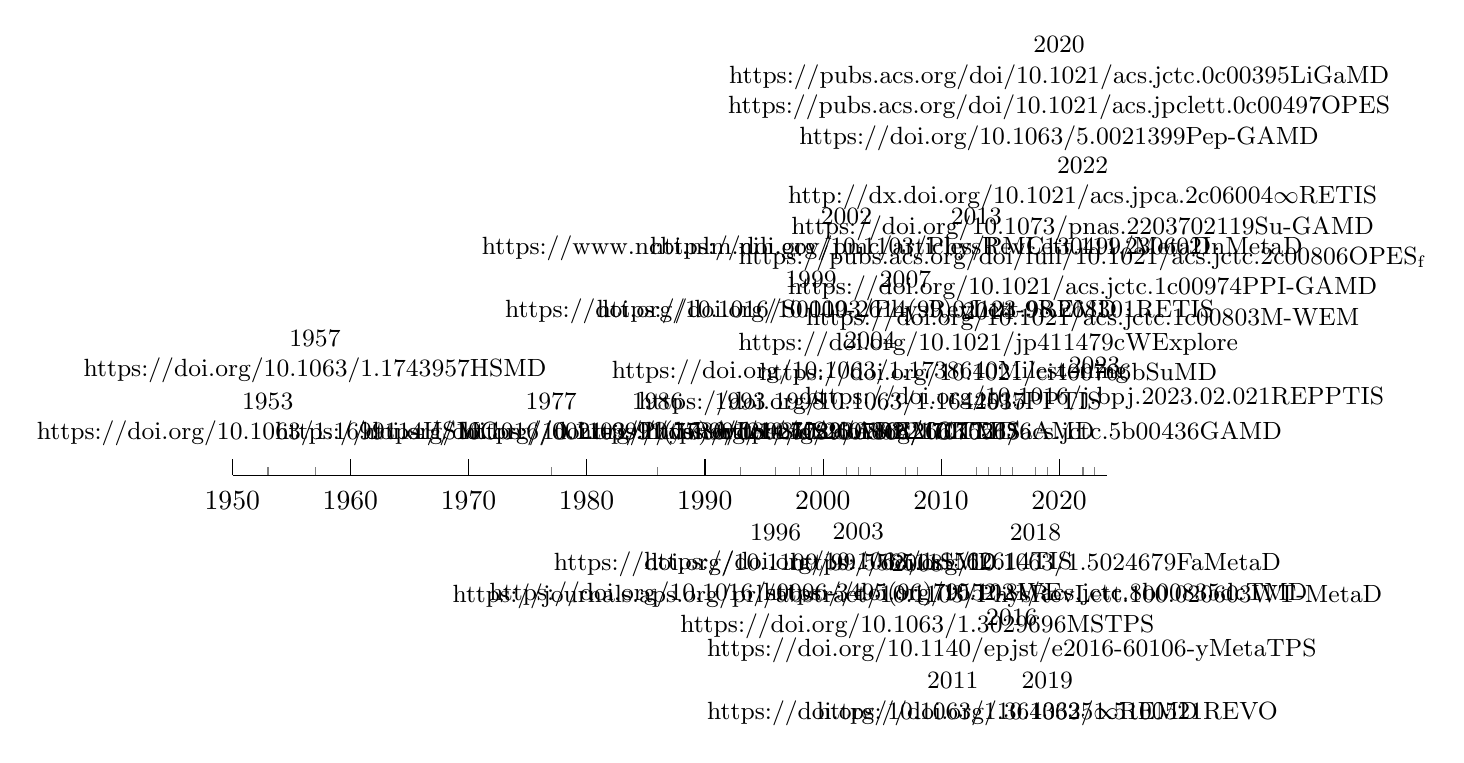
\begin{tikzpicture}[x=1.5cm,y=1cm]

% Timeline
\draw (195,0) -- (202.4,0);

% Events
\foreach \x/\dx/\dy/\y/\year/\event in {
195.3/0/0/0.01/1953/1953\\HCMC,
195.7/0/0/0.01/1957/1957\\HCMD,
197.7/0/0/0.01/1977/1977\\US,
198.6/0/0/0.01/1986/1986\\REMC,
199.3/0/0/0.01/1993/1993\\TMD,
199.6/0/0/0.01/1996/1996\\SMD\\WE,
199.8/0/0/0.01/1998/1998\\TPS,
199.9/0/0/0.01/1998/1998\\REMD,
200.2/0/0/0.01/2002/2002\\MetaD,
200.3/0/0/0.01/2003/2003\\TIS,
200.4/0/0/0.01/2004/2004\\AMD,
200.7/0/0/0.01/2004/2004\\RETIS,
200.8/0/0/0.01/2004/2004\\WT-MetaD,
201.3/0/0/0.01/2013/2013\\InMetaD,
201.4/0/0/0.01/2014/2014\\SuMD,
201.5/0/0/0.01/2015/2015\\GAMD,
201.6/0/0/0.01/2015/2015\\MetaTPS,
201.8/0/0/0.01/2018/2018\\WT-MetaD\\FaMetaD,
201.9/0/0/0.01/2018/2018\\REVO
202.0/0/0/0.01/2020/2020\\LiGaMD\\OPES,
202.2/0/0/0.01/2022/2022\\$\infty$RETIS\\OPES$_\mathrm{f}$,
202.3/0/0/0.01/2023/2023\\REPPTIS
}{
    \draw[color=gray] (\x,0+\dx) -- (\x, \y+0.10+\dy);
}
\foreach \x/\year in {195.0/1950,196.0/1960,197.0/1970,198.0/1980,199.0/1990,200.0/2000,201.0/2010,202.0/2020}{
 \draw (\x,0) node[below=0.2cm,,inner sep=0pt] {\colx{\year}} -- (\x,0.2);
}


\foreach \x/\y/\year/\event in {
195.3/0.05/k953/\colx{1953}\\\colx{\href{https://doi.org/10.1063/1.1699114}{HSMC}},
195.7/0.85/1957/\colx{1957}\\\colx{\href{https://doi.org/10.1063/1.1743957}{HSMD}},
197.7/0.05/1977/\colx{1977}\\\colx{\href{https://doi.org/10.1016/0021-9991(77)90121-8}{US}},
198.6/0.05/1986/\colx{1986}\\\colx{\href{https://doi.org/10.1103/PhysRevLett.57.2607}{REMC}},
199.3/0.05/1993/\colx{1993}\\\colx{\href{https://doi.org/10.1080/08927029308022170}{TMD}},
199.6/-2.00/1996/\colx{1996}\\\colx{\href{https://doi.org/10.1109/99.556511}{SMD}}\\\colx{\href{https://doi.org/10.1016/s0006-3495(96)79552-8}{WE}},
199.8/0.05/1998/\colx{1998}\\\colx{\href{https://doi.org/10.1039/A801266K}{TPS}},
199.9/1.6/1999/\colx{1999}\\\colx{\href{https://doi.org/10.1016/S0009-2614(99)01123-9}{REMD}},
200.2/2.4/2002/\colx{2002}\\\colx{\href{https://www.ncbi.nlm.nih.gov/pmc/articles/PMC130499/}{MetaD}},
200.3/-1.6/2003/\colx{2003}\\\colx{\href{https://doi.org/10.1063/1.1562614}{TIS}},
200.4/0.05/2004/\colx{2004}\\\colx{\href{https://doi.org/10.1063/1.1738640}{Milestoning}}\\\colx{\href{https://doi.org/10.1063/1.1644537}{PPTIS}}\\\colx{\href{https://doi.org/10.1063/1.1755656}{AMD}},
200.7/1.6/2007/\colx{2007}\\\colx{\href{https://doi.org/10.1103/PhysRevLett.98.268301}{RETIS}},
200.8/-2.4/2008/\colx{2008}\\\colx{\href{https://journals.aps.org/prl/abstract/10.1103/PhysRevLett.100.020603}{WT-MetaD}}\\\colx{\href{https://doi.org/10.1063/1.3029696}{MSTPS}},
201.1/-3.5/2008/\colx{2011}\\\colx{\href{https://doi.org/10.1063/1.3643325}{$\infty$REMD}},
201.3/2.4/2013/\colx{2013}\\\colx{\href{https://doi.org/10.1103/PhysRevLett.111.230602}{InMetaD}},
201.4/0.8/2014/\colx{2014}\\\colx{\href{https://doi.org/10.1021/jp411479c}{WExplore}}\\\colx{\href{https://doi.org/10.1021/ci400766b}{SuMD}},
201.5/0.05/2015/\colx{2015}\\\colx{\href{http://dx.doi.org/10.1021/acs.jctc.5b00436}{GAMD}},
201.6/-2.7/2016/\colx{2016}\\\colx{\href{https://doi.org/10.1140/epjst/e2016-60106-y}{MetaTPS}},
201.8/-2.0/2018/\colx{2018}\\\colx{\href{https://doi.org/10.1063/1.5024679}{FaMetaD}}\\\colx{\href{https://doi.org/10.1021/acs.jctc.8b00835}{dcTMD}},
201.9/-3.5/2019/\colx{2019}\\\colx{\href{https://doi.org/10.1063/1.5100521}{REVO}},
202.0/3.8/2020/\colx{2020}\\\colx{\href{https://pubs.acs.org/doi/10.1021/acs.jctc.0c00395}{LiGaMD}}\\\colx{\href{https://pubs.acs.org/doi/10.1021/acs.jpclett.0c00497}{OPES}}\\\colx{\href{https://doi.org/10.1063/5.0021399}{Pep-GAMD}},
202.2/1.5/2022/\colx{2022}\\\colx{\href{http://dx.doi.org/10.1021/acs.jpca.2c06004}{$\infty$RETIS}}\\\colx{\href{https://doi.org/10.1073/pnas.2203702119}{Su-GAMD}}\\\colx{\href{https://pubs.acs.org/doi/full/10.1021/acs.jctc.2c00806}{OPES$_\mathrm{f}$}}\\\colx{\href{https://doi.org/10.1021/acs.jctc.1c00974}{PPI-GAMD}}\\\colx{\href{https://doi.org/10.1021/acs.jctc.1c00803}{M-WEM}},
202.3/0.5/2023/\colx{2023}\\\colx{\href{https://doi.org/10.1016/j.bpj.2023.02.021}{REPPTIS}}
}{
    \node[above=0.2cm,align=center,font=\small] at (\x,\y) {\event};
}
\end{tikzpicture}
\end{document}
